\section{Ejercicio 4.}

Vamos a explicar brevemente la implementacion del sched\_rr. Para la parte privada mantuvimos dos vectores, donde el índice marca un cpu y el valor marca, en uno de los vectores los ticks restantes y en el otro los ticks por defecto. Por otro lado tenemos una cola de tareas a ejecutar. Además si una tarea esta ejecutandosé, bloqueandosé o fue terminada esta no va a estar en la misma. \\
El constructor, destructor, unblock y load de sched\_rr son tan simples que no hace falta explicación. Veamos la función tick.

\begin{Verbatim}[commandchars=\\\{\}]
\PY{k+kt}{int} \PY{n}{SchedRR}\PY{o}{:}\PY{o}{:}\PY{n}{tick}\PY{p}{(}\PY{k+kt}{int} \PY{n}{id\PYZus{}cpu}\PY{p}{,} \PY{k}{const} \PY{k}{enum} \PY{n}{Motivo} \PY{n}{m}\PY{p}{)} \PY{p}{\PYZob{}}
    \PY{k+kt}{int} \PY{n}{pid\PYZus{}ret} \PY{o}{=} \PY{n}{IDLE\PYZus{}TASK}\PY{p}{;}
    \PY{k+kt}{int} \PY{n}{pid\PYZus{}c} \PY{o}{=} \PY{n}{current\PYZus{}pid}\PY{p}{(}\PY{n}{id\PYZus{}cpu}\PY{p}{)}\PY{p}{;}
    \PY{k}{if} \PY{p}{(}\PY{n}{m} \PY{o}{=}\PY{o}{=} \PY{n}{TICK} \PY{o}{\PYZam{}}\PY{o}{\PYZam{}} \PY{n}{pid\PYZus{}c} \PY{o}{!}\PY{o}{=} \PY{n}{IDLE\PYZus{}TASK}\PY{p}{)} \PY{p}{\PYZob{}}
        \PY{n}{cpu\PYZus{}quantum}\PY{p}{[}\PY{n}{id\PYZus{}cpu}\PY{p}{]}\PY{o}{\PYZhy{}}\PY{o}{\PYZhy{}}\PY{p}{;}
        \PY{k}{if} \PY{p}{(}\PY{n}{cpu\PYZus{}quantum}\PY{p}{[}\PY{n}{id\PYZus{}cpu}\PY{p}{]} \PY{o}{=}\PY{o}{=} \PY{l+m+mi}{0} \PY{o}{\PYZam{}}\PY{o}{\PYZam{}} \PY{o}{!}\PY{n}{q}\PY{p}{.}\PY{n}{empty}\PY{p}{(}\PY{p}{)}\PY{p}{)} \PY{p}{\PYZob{}}
            \PY{n}{q}\PY{p}{.}\PY{n}{push}\PY{p}{(}\PY{n}{pid\PYZus{}c}\PY{p}{)}\PY{p}{;}
            \PY{n}{pid\PYZus{}ret} \PY{o}{=} \PY{n}{q}\PY{p}{.}\PY{n}{front}\PY{p}{(}\PY{p}{)}\PY{p}{;}
            \PY{n}{q}\PY{p}{.}\PY{n}{pop}\PY{p}{(}\PY{p}{)}\PY{p}{;}
            \PY{n}{cpu\PYZus{}quantum}\PY{p}{[}\PY{n}{id\PYZus{}cpu}\PY{p}{]} \PY{o}{=} \PY{n}{def\PYZus{}quantum}\PY{p}{[}\PY{n}{id\PYZus{}cpu}\PY{p}{]}\PY{p}{;}
        \PY{p}{\PYZcb{}} \PY{k}{else} \PY{p}{\PYZob{}}
            \PY{n}{pid\PYZus{}ret} \PY{o}{=} \PY{n}{pid\PYZus{}c}\PY{p}{;}
            \PY{k}{if} \PY{p}{(}\PY{o}{!}\PY{n}{cpu\PYZus{}quantum}\PY{p}{[}\PY{n}{id\PYZus{}cpu}\PY{p}{]}\PY{p}{)} \PY{n}{cpu\PYZus{}quantum}\PY{p}{[}\PY{n}{id\PYZus{}cpu}\PY{p}{]} \PY{o}{=} \PY{n}{def\PYZus{}quantum}\PY{p}{[}\PY{n}{id\PYZus{}cpu}\PY{p}{]}\PY{p}{;}
        \PY{p}{\PYZcb{}}
    \PY{p}{\PYZcb{}} \PY{k}{else} \PY{p}{\PYZob{}}
        \PY{k}{if} \PY{p}{(}\PY{o}{!}\PY{n}{q}\PY{p}{.}\PY{n}{empty}\PY{p}{(}\PY{p}{)}\PY{p}{)} \PY{p}{\PYZob{}}
            \PY{n}{pid\PYZus{}ret} \PY{o}{=} \PY{n}{q}\PY{p}{.}\PY{n}{front}\PY{p}{(}\PY{p}{)}\PY{p}{;}
            \PY{n}{q}\PY{p}{.}\PY{n}{pop}\PY{p}{(}\PY{p}{)}\PY{p}{;}
            \PY{n}{cpu\PYZus{}quantum}\PY{p}{[}\PY{n}{id\PYZus{}cpu}\PY{p}{]} \PY{o}{=} \PY{n}{def\PYZus{}quantum}\PY{p}{[}\PY{n}{id\PYZus{}cpu}\PY{p}{]}\PY{p}{;}
        \PY{p}{\PYZcb{}}
    \PY{p}{\PYZcb{}}
    \PY{k}{return} \PY{n}{pid\PYZus{}ret}\PY{p}{;}
\PY{p}{\PYZcb{}}
\end{Verbatim}

Como se ve lo que hacemos es fijarnos si actualmente esta corriendo una tarea idle o pidió un block/exit. En tal caso lo único que hace falta es intentar cargar una nueva tarea al cpu, de no poder hacerlo, porque no hay tareas en la cola, dejamos la idle. Si era un tick y además no era la tarea idle, vemos si fue el ultimo tick, en tal si hay álguna tarea en la cola de procesos, la cargamos, y sino devolvemos la idle.

Luego para probar que andaba corrimos el scheduler con el loteEj5.tsk que es

\begin{Verbatim}
TaskBatch 12 4
TaskCPU   34
TaskBatch 25 3
TaskCPU   8
\end{Verbatim}

Obteniendo

\begin{figure}[h]
    \centerline{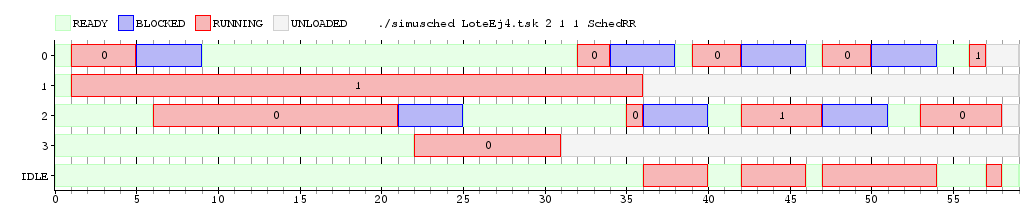
\includegraphics[scale=0.55]{images/imgEjercicio4}}
    \caption{Round Robin Lote4.}
\end{figure}

